\section{Components and processes for introducing new data, analytic tools, documents}\label{class}

\subsection{Contributions and review}\label{contributions-and-review}

Proposed contributions to Bioconductor's ecosystem of software packages,
data resources, and documentation are registered at
\begin{verbatim}
https://github.com/bioconductor/contributions/issues 
\end{verbatim}
Contributors
identify a public github.com repository that houses
their software, or some durable open data repository
for a data contribution. The contributor
provides schematized information on format, licensing, and commitment
to maintenance of the contributed resource. After a series of
automated and manual verification steps, the contributed
resource enters the review process.

An example under review in December 2023 is the ``methodical''
package, submitted 27 September 2023. The issue number
at the contributions site is 3169. This contribution is of
particular interest as it addresses new data resources from
whole genome and reduced representation bisulfite sequencing
experiments. Specifics on these high-resolution studies
of DNA methylation
in a variety of clinical situtions are given below.

\subsection{Data structures}\label{data-structures}

Inheritance is a key feature of object-oriented programming (OOP) that allows us to define a new class out of existing classes and add new features, which provides reusability of code. Inheritance carries over attributes and methods defined for base classes; `Attributes' are variables that are bound in a class. They are used to define behavior and methods for objects of that class. `Methods' are functions defined within a class that receive an instance of the class, conventionally called self, as the first argument. The attributes defined for a base class will automatically be present in the derived class, and the methods for the base class will work for the derived class. The R programming language has three different class systems: S3, S4, and Reference. Inheritance in S3 classes does not have any fixed definition, and hence attributes of S3 objects can be arbitrary. Derived classes, however, inherit the methods defined for the base class. Inheritance in S4 classes is more structured, and derived classes inherit both attributes and methods of the parent class. Reference classes are similar to S4 classes, but they are mutable and have reference semantics.

S4 classes are used extensively in Bioconductor to create data structures that store complex information, such as biological assay data and metadata, in one or more slots. The entire structure can then be assigned to an R object, and the types of information in each slot of the object are tightly controlled. S4 generics and methods define functions that can be applied to these objects, providing a rich software development infrastructure while ensuring interoperability, reusability, and efficiency.

Bioconductor have established Bioconductor classes to represent different types of biological data. Data and tools distributed through Bioconductor adopt Bioconductor classes, providing convenient methods and improving usability and interoperability within the Bioconductor ecosystem.

\begin{table}
\caption{Overview of key datatypes and associated classes in Bioconductor.}
\begin{tabular}[t]{ll}
\toprule
Data Types & Bioconductor Classes\\
\midrule
Genomic coordinates (1-based, closed interval) & GRanges\\
Groups of genomic coordinates & GRangesList\\
Ragged genomic coordinates & RaggedExperiment\\
Gene sets & GeneSet\\
Rectangular Features x samples & SummarizedExperiment\\
\addlinespace
Multi-omics data & MultiAssayExperiment\\
Single-cell data & SingleCellExperiment\\
Spatial Transcriptomics & SpatialExperiment\\
Mass spectrometry data & Spectra\\
\bottomrule
\end{tabular}
\end{table}

The GRanges class represents a collection of genomic ranges and associated annotations. Each element in the vector represents a set genomic ranges in terms of the sequence name (seqnames, typically the chromosome), start and end coordinates (ranges, as an IRanges object), strand (strand, either positive, negative, or unstranded), and optional metadata columns (e.g., exon\_id and exon\_name in the below).

\begin{verbatim}
GRanges object with 4 ranges and 2 metadata columns:
      seqnames            ranges strand |   exon_id       exon_name
         <Rle>         <IRanges>  <Rle> | <integer>     <character>
  [1]        X 99883667-99884983      - |    667145 ENSE00001459322
  [2]        X 99885756-99885863      - |    667146 ENSE00000868868
  [3]        X 99887482-99887565      - |    667147 ENSE00000401072
  [4]        X 99887538-99887565      - |    667148 ENSE00001849132
  -------
  seqinfo: 722 sequences (1 circular) from an unspecified genome
\end{verbatim}

The GRangesList object serves as a container for genomic features consisting of multiple
ranges that are grouped by a parent features, such as spliced transcripts that are
comprised of exons. A GRangesList object behaves like a list and many of the same
methods for GRanges objects are available for GRangesList object as well.

The SummarizedExperiment class (see Figure \ref{fig:sesc} is a matrix-like container, where rows represent features of interest (e.g., genes, transcripts, exons, etc.) and columns represent samples. The attributes of this object include experimental results (in assays), information on observations (in rowData) and samples (in colData), and additional metadata (in metadata). SummarizedExperiment objects can simultaneouly manage several experimental results as long as they are of the same dimensions. The best benefit of using SummarizedExperiment class is the coordination of the metadata and assays when subsetting. SummarizedExperiment is similar to the historical ExpressionSet class, but more flexible in its row information, allowing both GRanges and DataFrames. ExpressionSet object can be easily converted to SummarizedExperiment.

RangedSummarizedExperiment inherits the SummarizedExperiment class, with the extended capability of storing genomic ranges (as a GRanges or GRangesList object) of interest instead of a DataFrame (S4-class objectcs similar to data.frame) of features in rows.

The MultiAssayExperiment class (presented above in
Figure \ref{fig:masc}) is modeled after the SummarizedExperiment class.
A MultiAssayExperiment instance \texttt{M} can be
filtered as a three-dimensional array.
When \texttt{G} is a vector of feature identifiers,
\texttt{C} a vector of sample identifiers, and \texttt{E} a
vector of experiment names, then \texttt{M{[}G, C, E{]}} is
a MultiAssayExperiment with content restricted to the
requested features, samples, and experiments. The MultiAssayExperiment
package includes tooling to convert data content to ``long'' or
``wide'' formats. In long format, each element of the assay array occupies
a row, accompanied by metadata associated with the element.
In wide format, each sample occupies a row, accompanied by all
assocated assay and metadata elements.

\subsection{Out-of-memory data representation strategies}\label{out-of-memory-data-representation-strategies}

We return to the ``methodical'' package
submission mentioned above.
A number of whole-genome bisulfite sequencing experiments on
tumors from various anatomic sites are available
in ExperimentHub.
Metadata in that package shows that the datasets
are large, ranging from 2-40 gigabytes. One smaller
dataset is provided for illustration.

%\begin{Shaded}
%\begin{Highlighting}[]
%\KeywordTok{library}\NormalTok{(TumourMethData)}
%\NormalTok{demm =}\StringTok{ }\KeywordTok{download\_meth\_dataset}\NormalTok{(}\StringTok{"mcrpc\_wgbs\_hg38\_chr11"}\NormalTok{)}
%\CommentTok{\#\# [1] "A HDF5 SummarizedExperiment is already present in /home/vincent/TEMP/RtmpIQh7nv/mcrpc\_wgbs\_hg38\_chr11 and is being returned"}
%\NormalTok{demm}
%\CommentTok{\#\# class: RangedSummarizedExperiment }
%\CommentTok{\#\# dim: 1333114 100 }
%\CommentTok{\#\# metadata(5): genome is\_h5 ref\_CpG chrom\_sizes descriptive\_stats}
%\CommentTok{\#\# assays(2): beta cov}
%\CommentTok{\#\# rownames: NULL}
%\CommentTok{\#\# rowData names(0):}
%\CommentTok{\#\# colnames(100): DTB\_003 DTB\_005 ... DTB\_265 DTB\_266}
%\CommentTok{\#\# colData names(4): metastatis\_site subtype age sex}
%\KeywordTok{rowRanges}\NormalTok{(demm)}
%\CommentTok{\#\# GRanges object with 1333114 ranges and 0 metadata columns:}
%\CommentTok{\#\#             seqnames    ranges strand}
%\CommentTok{\#\#                \textless{}Rle\textgreater{} \textless{}IRanges\textgreater{}  \textless{}Rle\textgreater{}}
%\CommentTok{\#\#         [1]    chr11     60077      *}
%\CommentTok{\#\#         [2]    chr11     60088      *}
%\CommentTok{\#\#         [3]    chr11     60365      *}
%\CommentTok{\#\#         [4]    chr11     60941      *}
%\CommentTok{\#\#         [5]    chr11     60979      *}
%\CommentTok{\#\#         ...      ...       ...    ...}
%\CommentTok{\#\#   [1333110]    chr11 135076482      *}
%\CommentTok{\#\#   [1333111]    chr11 135076496      *}
%\CommentTok{\#\#   [1333112]    chr11 135076502      *}
%\CommentTok{\#\#   [1333113]    chr11 135076507      *}
%\CommentTok{\#\#   [1333114]    chr11 135076510      *}
%\CommentTok{\#\#   {-}{-}{-}{-}{-}{-}{-}}
%\CommentTok{\#\#   seqinfo: 25 sequences from an unspecified genome; no seqlengths}
%\KeywordTok{names}\NormalTok{(}\KeywordTok{colData}\NormalTok{(demm))}
%\CommentTok{\#\# [1] "metastatis\_site" "subtype"         "age"             "sex"}
%\KeywordTok{table}\NormalTok{(demm}\OperatorTok{$}\NormalTok{metastatis\_site)}
%\CommentTok{\#\# }
%\CommentTok{\#\#       Bone      Liver Lymph\_node      Other }
%\CommentTok{\#\#         43         11         38          8}
%\end{Highlighting}
%\end{Shaded}

\begin{shaded}
\begin{verbatim}
library(TumourMethData)
demm = download_meth_dataset("mcrpc_wg ..." ... [TRUNCATED] 
demm
## class: RangedSummarizedExperiment 
## dim: 1333114 100 
## metadata(5): genome is_h5 ref_CpG chrom_sizes descriptive_stats
## assays(2): beta cov
## rownames: NULL
## rowData names(0):
## colnames(100): DTB_003 DTB_005 ... DTB_265 DTB_266
## colData names(4): metastatis_site subtype age sex
rowRanges(demm)
## GRanges object with 1333114 ranges and 0 metadata columns:
##             seqnames    ranges strand
##                <Rle> <IRanges>  <Rle>
##         [1]    chr11     60077      *
##         [2]    chr11     60088      *
##         [3]    chr11     60365      *
##         [4]    chr11     60941      *
##         [5]    chr11     60979      *
##         ...      ...       ...    ...
##   [1333110]    chr11 135076482      *
##   [1333111]    chr11 135076496      *
##   [1333112]    chr11 135076502      *
##   [1333113]    chr11 135076507      *
##   [1333114]    chr11 135076510      *
##   -------
##   seqinfo: 25 sequences from an unspecified genome; no seqlengths
names(colData(demm))
## [1] "metastatis_site" "subtype"         "age"             "sex"            
table(demm$metastatis_site)
##      Bone      Liver Lymph_node      Other 
##        43         11         38          8 
\end{verbatim}
\end{shaded}


References to \texttt{demm} involve an 800MB excerpt of a
prostate cancer atlas with a
storage footprint of 40GB.
Ideally,
queries about particular genomic
regions on particular samples, whole-sample statistical summaries,
and searches for patterns can be carried out without
specific accommodation of the data size or representation.
The DelayedArray package helps pursue this aim. We'll illustrate
by interrogating the prostate cancer WGBS data for ``beta''
(fraction of locus that is methylated) values in the vicinity of
gene ATM.

\begin{shaded}
\begin{verbatim}
library(EnsDb.Hsapiens.v86)
gg = genes(EnsDb.Hsapiens.v86)
# get gene addresses
atmpos = gg[gg$gene_name == "ATM" &
gg$gene_biotype == "protein_coding"] # filter to ATM
seqlevelsStyle(atmpos) = "UCSC"
assay(subsetByOverlaps(demm, atmpos+1e6))
## <18110 x 100> DelayedMatrix object of type "double":
##          DTB_003 DTB_005 DTB_008 ... DTB_265 DTB_266
##     [1,]  0.1053  0.7660  0.9206   .  0.6944  0.9412
##     [2,]  0.4062  0.9091  0.9318   .  0.5676  1.0000
##     [3,]  0.1379  0.0000  0.7400   .  0.4643  0.9231
##     [4,]  0.2308  0.9231  0.9149   .  0.8929  0.9286
##     [5,]  0.1481  0.8500  0.8864   .  0.8710  0.9762
##      ...       .       .       .   .       .       .
## [18106,]  0.4138  0.3143  0.3208   . 0.17647 0.10000
## [18107,]  0.2727  0.2745  0.4143   . 0.22500 0.32500
## [18108,]  0.2258  0.4800  0.5775   . 0.08889 0.25000
## [18109,]  0.5278  0.7059  0.8088   . 0.55263 0.97561
## [18110,]  0.2778  0.3137  0.6957   . 0.52632 0.35714
\end{verbatim}
\end{shaded}


The numeric values presented above are just the
``corners'' of the associated array, presented as a ``check''
on the content requested. Transfer of array content to
the CPU for numerical analysis only occurs on demand,
which can be tailored to the quantity of RAM available
at analysis time.

\subsection{Quality assessment of Bioconductor resources}\label{quality-assessment-of-bioconductor-resources}

Figure \ref{fig:qapic} is an overview of the periodic ecosystem
testing process for Bioconductor software packages in the
release branch. All Bioconductor
and CRAN packages on which they depend are present and are updated
on change to sources.

\begin{figure}
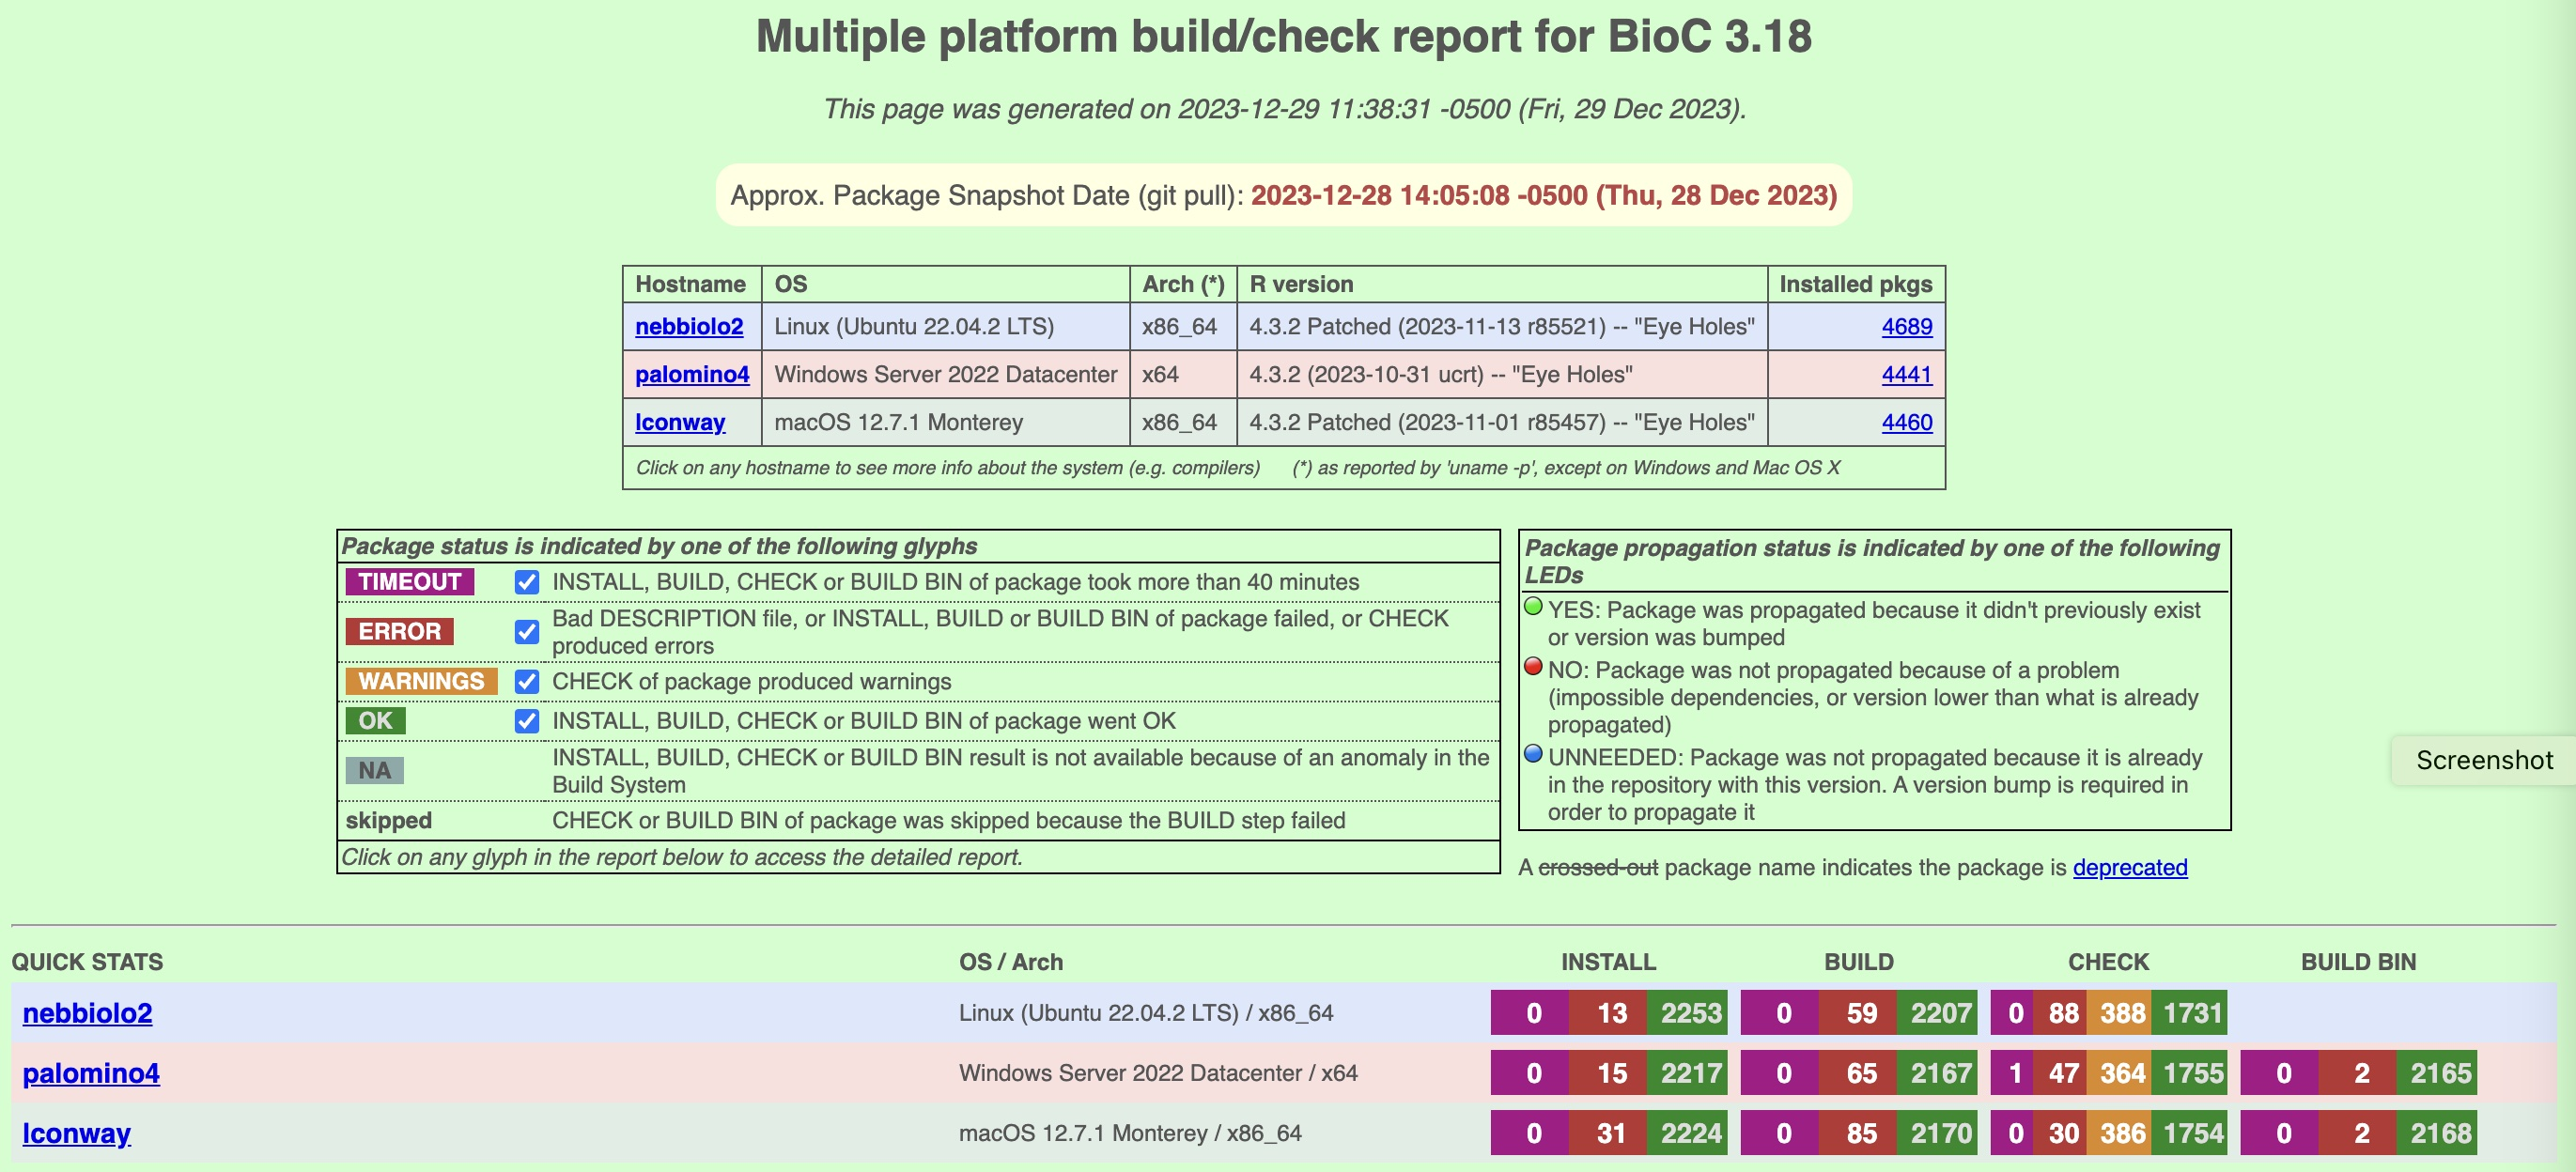
\includegraphics[width=1.21\linewidth,]{QApage} \caption{Build report for Bioc 3.18, 12-29-2023.}\label{fig:qapic}
\end{figure}

The project distributes source tarballs for Linux-like systems, and
compiled binaries for MacOS and Windows. Numbers in red boxes indicate
failures to install, build, or check. Failure events are
frequently platform-specific; full logs are provided
on the build report pages to help developers isolate and fix
build and check errors. When failures are persistent, developers
are contacted by core. If contact cannot be made and failures
continue, packages are deprecated for at least one release, and
then removed.

\section{Pedagogics and workforce development}\label{pedagogics-and-workforce-development}

The Bioconductor project has undertaken a number
of initiatives to support growth of the
scientific workforce's capacity to efficiently
integrate and interpret
genome-scale experiments.

\begin{itemize}
\item
  \textbf{Partnering with The Carpentries.} The Carpentries \url{https://carpentries.org} is a non-profit organization focused on teaching programming
  and data science to researchers. The organization defines ``good
  practices in lesson design and development, and open source
  collaboration skills''. Bioconductor community members have
  created bioc-intro, bioc-project, and bioc-rnaseq repositories
  using The Carpentries Incubator template. This arrangement helps
  Bioconductor create and manage a ``train the trainer'' process
  according to tested pedagogical principles.
\item
  \textbf{Curating monographs for topics in genomic data science.} The
  breadth of Bioconductor resources for genomics, combined with the
  energetic approach to software and annotation upkeep in the project,
  empowers Bioconductor developers to produce unified, wide-ranging,
  computable documents on topics of interest to the broader
  cancer genomics community. Books currently available
  at bioconductor.org include OSCA (Orchestrating Single Cell Analysis
  with Bioconductor), SingleRBook (Assigning cell types with SingleR),
  csawBook (Analysis of ChIP-seq data), OHCA (Orchestrating Hi-C
  Analysis with Bioconductor) and R for Mass Spectrometry. Very
  recently, Jacques Serizay of Institut Pasteur has contributed
  a book authoring framework called BiocBook. This transforms documents
  marked up in Posit's quarto format into web-based books backed up by Docker
  containers and maintained with templated GitHub actions. The
  OHCA book is produced and managed with BiocBook.
\item
  \textbf{A system for authoring and deploying interactive workshops.}
\end{itemize}

Figure \ref{fig:wssc} gives an overview of the resources and
objectives of the system underlying \url{workshop.bioconductor.org}.
Given a kubernetes-enabled cluster
the workshop system assembles

\begin{itemize}
\tightlist
\item
  compute and storage elements,
\item
  static components (training texts and shareable data),
\item
  development environments (containers with all runtime elements
  required to compiled code, conduct analyses, communicate with GPUs).
\end{itemize}

\begin{figure}
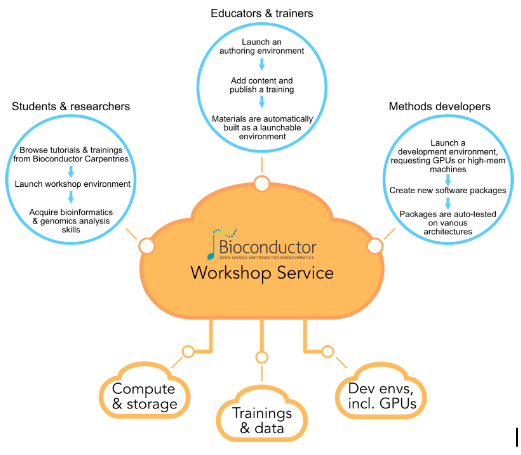
\includegraphics[width=0.8\linewidth,]{WorkshopSCHEMA} \caption{Workshop.bioconductor.org schematic.}\label{fig:wssc}
\end{figure}

A lightly customized deployment of the Galaxy system (usegalaxy.org)
is used to deal with authentication
and process initiation and termination.

This system has been used to serve interactive workshops in a number
of international conferences. Content in R markdown or quarto
can be produced by anyone interested in offering a workshop, and
the ``BiocWorkshopSubmit'' app at workshop.bioconductor.org
can be used to identify new content to the system. Markdown
documents will be analyzed to determine what resources are needed
for the containerization of workshop software and data components,
and the container will be created and registered at the GitHub
Container Registry. Arrangements to deploy the workshop over
a given calendar period can be made with Bioconductor core. The
workshop container can be used to conduct the workshop on any
system with a Docker client.

\section{Conclusions and paths forward}\label{conclusions-and-paths-forward}

We have described several aspects of
Bioconductor's approach to ecosystem management for cancer
genomics data science resources. In light of
the dynamism
of biotechnological innovation, it is clear that the project
must anticipate change. But it is challenging to introduce
changes to processes on which a very large community depends
for their daily research work. Commitments to supporting reproducible
research entail that Bioconductor preserves decades worth of images
of software and data for immediate retrieval via
web request by parties unknown
to the project.

We'll conclude this report with a few observations on
general paths that the project is likely to take that
should have favorable consequences to researchers in
cancer genomics.

\begin{itemize}
\item
  \textbf{Language-agnostic data and annotation} The \texttt{alabaster.*} packages
  introduced in Bioconductor 3.17 are designed to convert existing
  Bioconductor data structures to formats that are more readily ingested
  by software in other languages. Thus the \texttt{alabaster.mae}
  package will convert a MultiAssayExperiment into a collection
  of files of metadata (serialized in JSON), sample-level data
  (serialized as CSV), and assay data (serialized to HDF5).
\item
  \textbf{Zero-configuration genomic analysis environments} Users
  of Docker containers have long been able to take advantage of
  Bioconductor containers pre-populated with Rstudio and runtime
  resources to support installation of any desired software packages.
  The bioc2u system (\url{https://github.com/bioconductor/bioc2u}) in conjunction
  with r2u (\url{github.com/eddelbuettel/r2u}) introduces the
  availability of Debian packages for all Bioconductor packages,
  made available in a CRAN-like repository. Given a system running
  Ubuntu 22 or 20, the apt package manager will resolve any package
  requests with tested, fully linked binary packages. Users do not
  have to perform any configuration or compilation of system
  utilities or package code. This practice can greatly reduce
  resource consumption that occurs when individuals or
  workflow systems need to compile
  every package and its dependencies to perform analyses.
\item
  \textbf{Computation at the data} Several members of Bioconductor's
  development core are on the technical development team of
  NHGRI's Analysis and Visualization Laboratory (AnVIL). The aim
  of this project is to overthrow the prevalent model of downloading data for
  local analysis. AnVIL mobilizes commercial cloud computing and
  storage to support truly elastic genomic analysis -- create and
  pay for only the computation you need. The basic
  strategy is described in Schatz et al. (\protect\hyperlink{ref-Schatz2022}{2022}). This system was
  used in the production of the Telomere-to-Telomere
  genome build, see Aganezov et al. (\protect\hyperlink{ref-Aganezov2022}{2022}).
\end{itemize}

We hope that the project can continue to support researchers in cancer
genomics for another 20 years!

%\section{Acknowledgments}\label{acknowledgments}
%
%%This work was supported in part by NIH NCI 3U24CA180996-10S1, NHGRI 5U24HG004059-18, and NSF ACCESS allocation BIR190004.
